\documentclass[../ai_in_finance]{subfiles}
\usepackage[margin=1in]{geometry}
\usepackage{tikz}
\usetikzlibrary{positioning}
\usepackage{amsmath}
\usepackage{amssymb}
\usepackage{booktabs}
\usepackage{draftwatermark}

\SetWatermarkText{WSuo@Queensu.ca}
\SetWatermarkScale{1.4}
\SetWatermarkColor{gray!35}
\SetWatermarkAngle{45}

\usepackage{makeidx}
\makeindex

\begin{document}

\chapter{Credit Risk Modeling}

\section{Introduction}

Chapter 8 developed the standard toolkit for market risk, Value at Risk\index{Value at Risk (VaR)}, Expected Shortfall, and the volatility and correlation machinery behind them. This chapter turns to a related but genuinely distinct problem: credit risk, the risk that a counterparty, whether a bond issuer, a loan borrower, or a derivatives counterparty, fails to meet a contractual obligation. Where market risk asks how much a position's \emph{value} could move, credit risk asks whether a counterparty will \emph{pay at all}, a binary event with its own probability, its own severity once it occurs, and its own regulatory and modeling apparatus, probability of default, loss given default, credit scoring, structural models, and rating systems, developed in full below.

The chapter proceeds from the single-borrower case to the whole-portfolio case, mirroring the logic Chapter 8 used for individual positions versus an entire book. It begins with the three-component decomposition of expected loss and what drives each component, moves through three genuinely distinct ways of estimating a borrower's probability of default, a statistical model fit to historical data, a structural model that reads default risk directly out of market prices, and a market-implied approach that reads it out of credit derivative spreads, and then extends single-borrower ratings into multi-year transition matrices. The chapter closes by moving from a single loan to an entire portfolio, where the correlation between borrowers' defaults, not just their individual probabilities, becomes the dominant driver of extreme loss, a theme illustrated concretely both by a worked single-factor model and by a real historical episode in which underestimating exactly that correlation contributed to a systemic financial crisis.

One worked example runs through much of the chapter: a small loan portfolio that reuses the credit-risk-adjusted bond from Chapter 5 and the loan dataset from Chapter 6, extending both into a full treatment of expected loss, credit scoring, and portfolio credit risk. As in earlier chapters, every numerical claim below was computed in Python first and is reproduced exactly in the companion notebook.

\section{Credit Risk Fundamentals: Expected Loss}\index{Credit Risk Fundamentals: Expected Loss}
\label{sec:credit-risk-fundamentals}

Suppose a bank holds a bond and wants a single number summarizing how much of that exposure it should expect to lose to default, on average across many similar bonds, well before knowing whether this particular one actually defaults. Credit risk is conventionally decomposed into three components whose product answers exactly this, giving the expected loss on a credit exposure:
\begin{equation*}
\text{Expected Loss} = \text{PD} \times \text{LGD} \times \text{EAD},
\end{equation*}
where PD is the probability of default\index{Probability of Default (PD)} over the relevant horizon (typically one year), LGD is the loss given default\index{Loss Given Default (LGD)}, the fraction of the exposure not recovered after default, and EAD is the exposure at default\index{Exposure at Default (EAD)}, the dollar amount outstanding at the time of default (which can differ from the current balance for instruments like credit lines that can be drawn down further before default). Recall the corporate bond from Chapter 5's discussion of pricing default risk: face value \$1,000, one-year default probability $\text{PD}=3\%$, and a recovery rate of 40\% of face value, so $\text{LGD} = 1 - 0.40 = 60\%$. Treating the full face value as the exposure at default, $\text{EAD}=\$1{,}000$, the expected loss is
\begin{equation*}
\text{Expected Loss} = 0.03 \times 0.60 \times 1{,}000 = \$18.
\end{equation*}
Figure~\ref{fig:el_decomposition} lays out this same decomposition as a pipeline, since the rest of this chapter is organized around estimating each of these three inputs in turn, first PD (via logistic regression and, later, the Merton model), then LGD, then EAD.

\begin{figure}[htbp]
    \centering
    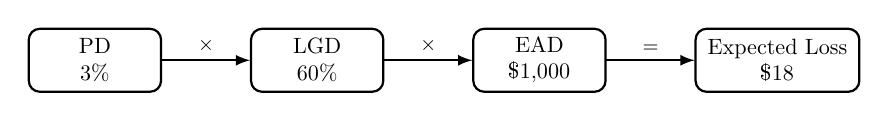
\begin{tikzpicture}[scale=0.8,transform shape,>=latex,thick,node distance=1.4cm]
        \node[draw,rounded corners,align=center,minimum width=2.1cm,minimum height=1.0cm] (pd) {PD\\$3\%$};
        \node[draw,rounded corners,align=center,minimum width=2.1cm,minimum height=1.0cm,right=of pd] (lgd) {LGD\\$60\%$};
        \node[draw,rounded corners,align=center,minimum width=2.1cm,minimum height=1.0cm,right=of lgd] (ead) {EAD\\\$1{,}000};
        \node[draw,rounded corners,align=center,minimum width=2.6cm,minimum height=1.0cm,right=of ead] (el) {Expected Loss\\\$18};
        \draw[->] (pd) -- node[above,font=\small] {$\times$} (lgd);
        \draw[->] (lgd) -- node[above,font=\small] {$\times$} (ead);
        \draw[->] (ead) -- node[above,font=\small] {$=$} (el);
    \end{tikzpicture}
    \caption{The expected-loss decomposition, applied to the Chapter 5 bond example. Each of PD, LGD, and EAD is estimated separately, using its own methods and data, before being combined into a single dollar figure.}
    \label{fig:el_decomposition}
\end{figure}
This is not a coincidence relative to Chapter 5's earlier calculation: that chapter found the bond's expected payoff to be \$982 against a promised \$1,000, and $1{,}000 - 982 = 18$ exactly, confirming that discounting the expected payoff and separately computing an expected loss are two equivalent ways of describing the same underlying credit risk. The practical distinction between the two framings is one of purpose rather than substance: the pricing framing of Chapter 5 asks ``what should this bond be worth today,'' while the expected-loss framing here asks ``how much of this exposure should a lender expect to lose, on average, and how much capital or loan-loss reserve should be held against that possibility,'' which is exactly the accounting and regulatory question addressed later in this chapter.

EAD is the least discussed of the three components in most introductory treatments, but it deserves its own worked example, since it is not simply ``the current balance'' whenever a borrower has undrawn credit available. Consider a committed revolving credit line with a \$500,000 total commitment, currently drawn to \$200,000, leaving \$300,000 undrawn. A defaulting borrower does not necessarily default with only the currently drawn amount outstanding; many borrowers draw down a credit line further as their financial condition deteriorates, often specifically because they are approaching default and want to secure cash while they still can, so exposure at default must account for some fraction of the undrawn commitment being drawn down before default actually occurs. Basel's standardized approach captures this with a credit conversion factor (CCF)\index{Credit Conversion Factor (CCF)}, the assumed fraction of the undrawn commitment that converts to drawn exposure by the time of default; for an unconditionally cancellable commercial credit line, a CCF of $50\%$ is a representative assumption, giving
\begin{equation*}
\text{EAD} = \text{Drawn} + \text{CCF} \times \text{Undrawn} = 200{,}000 + 0.50(300{,}000) = \$350{,}000,
\end{equation*}
75\% higher than the \$200,000 currently drawn balance, a difference the expected-loss formula above would otherwise have ignored entirely. This is precisely why credit lines and other commitment-based lending products carry more expected loss, for a given PD and LGD, than a fully drawn term loan of the same current balance, and why EAD, though it receives less modeling attention than PD or LGD in most textbook treatments, is estimated from its own dedicated historical dataset of drawn-versus-committed balances at the time of past defaults in any bank sophisticated enough to model it directly rather than relying on a regulatory CCF table.

\subsection{What Drives Loss Given Default}\index{What Drives Loss Given Default}
\label{sec:lgd-drivers}

PD tends to receive the most modeling attention, since it is the component most directly tied to the statistical and machine learning methods of Chapter 6, but LGD is just as consequential for expected loss and considerably harder to model well, since recovery outcomes depend on factors that are only observed after a default has already occurred. Seniority and collateral are the two most important drivers: a secured loan backed by specific collateral (real estate, equipment, inventory) typically recovers far more in default than an unsecured loan to the same borrower, since the lender has a direct claim on identifiable assets rather than competing with every other unsecured creditor for whatever remains. Seniority within the capital structure matters similarly: senior debt is repaid before subordinated debt in a bankruptcy, so a subordinated bondholder can face a substantially lower recovery rate than a senior bondholder to the very same defaulted issuer, even though both bondholders faced the identical probability of default.

Recovery rates are also cyclical in a way that compounds portfolio credit risk rather than diversifying it: during a recession, defaults become more frequent (PD rises) at precisely the same time that collateral values fall and distressed-asset markets become crowded with sellers (LGD rises too, since collateral fetches less in a forced sale), so PD and LGD are positively correlated across the credit cycle rather than independent, as this chapter's simplified expected-loss and economic-capital formulas implicitly assumed for tractability. A lender that estimates LGD from an average computed across a full credit cycle, rather than conditioning it on current or forecast economic conditions, will therefore tend to understate expected and unexpected losses specifically during the downturns when accurate loss estimates matter most, the same procyclicality theme raised elsewhere in this chapter.

Collateral coverage, the ratio of collateral value to loan balance, is directly estimable from a lender's own historical default data, and a simple linear regression already illustrates the qualitative pattern above numerically. Consider four hypothetical defaulted loans:
\begin{align*}
\text{Coverage} = 0.40, &\quad \text{Recovery} = 25\%, \\
\text{Coverage} = 0.60, &\quad \text{Recovery} = 45\%, \\
\text{Coverage} = 0.80, &\quad \text{Recovery} = 55\%, \\
\text{Coverage} = 1.20, &\quad \text{Recovery} = 75\%.
\end{align*} Fitting $\text{Recovery} = a + b\,(\text{Coverage})$ by ordinary least squares, exactly the estimation method Chapter 6 introduced,
\begin{equation*}
\hat b = \frac{\sum (x_i-\bar x)(y_i - \bar y)}{\sum (x_i - \bar x)^2} = 0.60, \qquad \hat a = \bar y - \hat b \bar x = 0.05,
\end{equation*}
so $\widehat{\text{Recovery}} = 0.05 + 0.60\,(\text{Coverage})$, with $R^2\approx0.969$, a strong linear fit given only four points. A loan with coverage exactly at $1.0$ (collateral value equal to the outstanding balance) has a predicted recovery of $0.05+0.60(1.0)=65\%$, implying $\text{LGD}=35\%$, meaningfully lower than the $60\%$ LGD assumed for the unsecured bond example running through this chapter, exactly the seniority-and-collateral effect described above made numerically concrete: a well-collateralized loan can have a substantially lower LGD than an otherwise identical unsecured exposure, and a lender with enough historical default data can estimate that relationship directly, the same regression logic Chapter 6 developed for very different financial applications, applied here to the loss side of credit risk rather than the default-probability side.

The high $R^2$ is worth treating with exactly the caution Chapter 6 raised about small samples, and computing the slope's standard error, following the same procedure applied to the credit-spread regression in that chapter, makes this concrete rather than merely qualitative. With only two degrees of freedom (four observations, two estimated parameters), $\text{SE}(\hat b) \approx 0.0756$, giving a $t$-statistic of $0.60/0.0756 \approx 7.94$ and a 95\% confidence interval for the slope of roughly $(0.27, 0.93)$. The slope is still statistically significant at conventional levels ($p\approx0.016$) despite the small sample, but the confidence interval itself is enormous relative to the point estimate: a true slope anywhere from $0.27$ to $0.93$ remains consistent with this data, meaning the predicted recovery rate at a coverage ratio of $1.0$ could plausibly range from roughly $32\%$ to $98\%$ once that parameter uncertainty is propagated through, an enormous practical range for a single reported LGD figure. This is precisely why a lender relying on a collateral-recovery regression estimated from only a handful of historical defaults should treat the fitted line as a useful starting point rather than a precise input, and should prioritize collecting more default history, or borrowing estimates from a broader industry dataset, before relying on it for capital or pricing decisions.

\subsection{Credit Stress Testing: Stressed PD and LGD}\index{Credit Stress Testing}
\label{sec:credit-stress-testing}

The procyclicality just described, PD and LGD both rising together in a downturn, is exactly what credit stress testing makes concrete. Rather than assuming the base-case PD and LGD estimated from calm, average conditions, a stress test recomputes expected loss under a specified adverse scenario, a recession, a sector-specific downturn, a sharp decline in collateral values, and asks how much larger expected loss becomes. Applying a stress scenario to the same bond from Section~\ref{sec:credit-risk-fundamentals}, doubling the default probability to a stressed $\text{PD}=8\%$ and raising loss given default to a stressed $\text{LGD}=70\%$ (reflecting weaker collateral values in a downturn, exactly the mechanism Section~\ref{sec:lgd-drivers} described), the stressed expected loss is
\begin{equation*}
\text{Expected Loss}^{\text{stress}} = 0.08 \times 0.70 \times 1{,}000 = \$56,
\end{equation*}
more than triple the base-case expected loss of \$18, even though neither input moved by an implausible amount on its own. This tripling is precisely why treating PD and LGD as independent, average-cycle constants, as this chapter's simpler formulas do for tractability, can be dangerously misleading for capital planning: a lender that reserves only against the calm-period expected loss will find its actual losses considerably larger than reserved for in exactly the scenario, a recession, when the shortfall matters most. Regulatory stress-testing exercises such as the Federal Reserve's CCAR, introduced from the market-risk side in Chapter 8, apply exactly this same stressed-PD-and-LGD logic across a bank's entire loan book, not just a single bond, projecting credit losses under a specified adverse macroeconomic scenario rather than the calm historical averages ordinary credit models are typically calibrated on.

\section{Credit Scoring with Logistic Regression}\index{Credit Scoring with Logistic Regression}
\label{sec:credit-scoring}

Expected loss requires an estimate of PD for each borrower, and Chapter 6 already introduced the standard statistical tool for producing one: logistic regression\index{logistic regression}, which models the probability of a binary outcome, here, default within the horizon, as a function of borrower characteristics. Recall the small loan dataset from Chapter 6's $K$-nearest neighbors\index{K-nearest neighbors (KNN)} example, with six applicants described by debt-to-income ratio and years of credit history. Fitting a logistic regression to that same dataset,
\begin{equation*}
\Pr(\text{Default}) = \frac{1}{1+e^{-z}}, \qquad z = -12.152 + 0.530\,(\text{Debt/Income}) - 0.231\,(\text{Credit History}),
\end{equation*}
gives coefficients that make economic sense: higher leverage increases the log-odds of default (positive coefficient), while a longer credit history reduces it (negative coefficient). Applying this to the same new applicant considered in Chapter 6 (debt-to-income of 28\%, 4 years of credit history),
\begin{equation*}
z = -12.152 + 0.530(28) - 0.231(4) \approx 1.761, \qquad \Pr(\text{Default}) = \frac{1}{1+e^{-1.761}} \approx 85.3\%.
\end{equation*}
This is consistent with, and considerably more precise than, the KNN classification from Chapter 6, which only produced a discrete ``predicted default'' label from a 2-to-1 majority vote among the three nearest neighbors; logistic regression instead reports a continuous probability, which is exactly the PD input Section~\ref{sec:credit-risk-fundamentals}'s expected-loss formula requires and which a simple majority-vote classifier cannot supply.

Lenders frequently rescale a model's output probability into a more interpretable credit score using a simple linear transformation, for example
\begin{equation*}
\text{Score} = 850 - 550 \times \Pr(\text{Default}),
\end{equation*}
chosen so that a default probability near 0 produces a score near 850 (the top of a typical consumer credit-score scale) and a default probability near 1 produces a score near 300 (the bottom). For the applicant above, $\text{Score} = 850 - 550(0.853) \approx 381$, a score that would place this applicant in a high-risk tier under most lenders' underwriting policies. The specific scaling constants are a business choice, not a statistical one, but the underlying logic, mapping a well-calibrated probability onto a scale that loan officers and borrowers can interpret intuitively, is universal, and connects directly back to the calibration discussion in Chapter 6: a credit score is only meaningful to the extent that the probability underlying it is itself accurately calibrated, not just useful for ranking applicants from safest to riskiest.

A subtler difficulty affects every credit scoring model built this way, regardless of how well it is fit or calibrated: a lender only observes loan performance for applicants it actually approved, since a rejected applicant never receives a loan and therefore never generates a default-or-no-default outcome to learn from. Training a model exclusively on approved applicants, exactly the six-applicant sample used throughout this section, means the model never sees how a rejected applicant, someone the previous underwriting policy already judged too risky, would actually have performed, a selection bias that can silently distort the fitted relationship between borrower characteristics and true default risk. Reject inference is the general name for techniques that attempt to correct for this, ranging from simple approaches (assigning rejected applicants an assumed outcome based on their characteristics) to more sophisticated statistical corrections that model the approval decision itself alongside the default outcome. None of these fixes is fully satisfying, since the true counterfactual, what would have happened had a rejected applicant been approved, is fundamentally unobservable, which is why reject inference remains an acknowledged, imperfect compromise in credit scoring practice rather than a solved problem, and why a credit model's performance on the population it was trained on can differ meaningfully from its performance on the full population of applicants it is actually used to screen. This is a credit-specific instance of a more general lesson from Chapter 6: a model is only as good as the data it learns from, and data generated by a decision process, here, a prior lending policy's approvals and rejections, is never a neutral, representative sample of the population that process was applied to.

\subsection{Validating a Credit Scoring Model: The Gini Coefficient and AUC}\index{Gini Coefficient}\index{AUC (Area Under the Curve)}
\label{sec:credit-model-validation}

Ranking applicants correctly from safest to riskiest is a distinct property from calibration, and it has its own standard validation metric in credit scoring: the area under the ROC curve (AUC), or equivalently the Gini coefficient, $\text{Gini} = 2\,\text{AUC}-1$, which rescales AUC so that a purely random ranking scores $0$ and a perfect ranking scores $1$. Both measure the same underlying question introduced more generally in Chapter 6: across every possible pair consisting of one defaulter and one non-defaulter, what fraction of the time does the model assign the defaulter a strictly higher predicted default probability? Applying the fitted logistic regression above to all six applicants in Chapter 6's Table 6.4, sorted by predicted default probability, gives the values in Table~\ref{tab:credit_auc}.

\begin{table}[htbp]
\centering
\caption{Predicted default probabilities for all six training applicants, sorted from highest to lowest risk}
\label{tab:credit_auc}
\begin{tabular}{lrrl}
\toprule
Applicant & Debt/income (\%) & $\Pr(\text{Default})$ & Actual outcome \\
\midrule
C & 40 & 0.9998 & Default \\
A & 35 & 0.9974 & Default \\
E & 30 & 0.9550 & Default \\
B & 20 & 0.0323 & No default \\
F & 18 & 0.0144 & No default \\
D & 15 & 0.0015 & No default \\
\bottomrule
\end{tabular}
\end{table}

Every one of the nine possible (defaulter, non-defaulter) pairs, three defaulters times three non-defaulters, is correctly ordered: each of C, A, and E's predicted probabilities exceeds each of B, F, and D's, so $\text{AUC}=9/9=1.0$ and $\text{Gini}=2(1.0)-1=1.0$, a perfect ranking. This is a genuine red flag rather than a cause for celebration, and for exactly the reason Chapter 6 raised repeatedly: this AUC is computed on the same six observations the model was fit to, with two features and six data points, so a perfect in-sample ranking is close to the least surprising outcome imaginable, not evidence the model would rank a new, out-of-sample applicant with anything like this accuracy. A real credit scoring model's AUC and Gini coefficient are only meaningful when computed on a genuinely held-out validation sample, following exactly the train-test discipline Chapter 6 developed at length, and an AUC this close to a perfect score on such a small training sample is itself a warning sign of overfitting to memorize, rather than a property to report proudly in a model validation document.

\section{Structural Credit Models: The Merton Model}\index{Structural Credit Models: The Merton Model}
\label{sec:merton-model}

Logistic regression estimates PD statistically, from historical data on borrower characteristics and past defaults. An entirely different approach, due to Merton (1974), estimates PD directly from market prices using an insight that connects directly back to the option pricing machinery of Chapter 5: a firm's equity can be modeled as a call option on the firm's assets, with the face value of its debt playing the role of the strike price.

The intuition is precise, not merely metaphorical. Shareholders have limited liability: if a firm's assets are worth more than its debt obligations at maturity, shareholders receive the difference (assets minus debt); if assets are worth less than the debt, shareholders receive nothing and the firm defaults, with bondholders taking control of the (insufficient) assets instead. This is exactly the payoff structure $\max(V_T - D, 0)$ of a European call option with the firm's asset value $V_T$ playing the role of the underlying price and the debt's face value $D$ playing the role of the strike, so the Black-Scholes-Merton\index{Black-Scholes-Merton Model} formula from Chapter 5 applies directly, with the firm's asset value in place of a stock price and its asset volatility in place of $\sigma$:
\begin{equation*}
E_0 = V_0 N(d_1) - D e^{-rT} N(d_2), \qquad d_1 = \frac{\ln(V_0/D) + (r + \sigma_V^2/2)T}{\sigma_V\sqrt{T}}, \qquad d_2 = d_1 - \sigma_V\sqrt{T},
\end{equation*}
where $E_0$ is the market value of equity, $V_0$ is the (unobserved) market value of the firm's assets, and $\sigma_V$ is asset volatility. The probability of default, the probability that assets fall below the debt's face value at maturity, is exactly the risk-neutral probability that the option expires out of the money,
$$\Pr(\text{Default}) = N(-d_2),$$
the same $N(-d_2)$ term that appeared when Chapter 5 priced a European put. Figure~\ref{fig:merton_payoff} draws this payoff structure directly: equity holders receive nothing if the firm's assets are worth less than its debt at maturity, and the excess above debt otherwise, exactly a call option's hockey-stick payoff with the debt's face value playing the role of the strike price.

\begin{figure}[htbp]
    \centering
    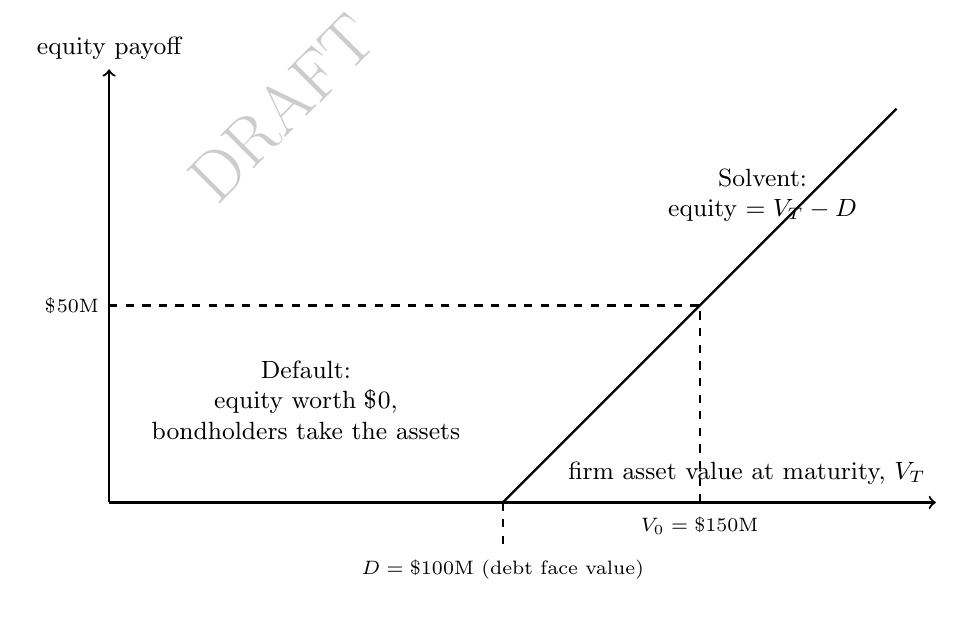
\begin{tikzpicture}[thick]
        \draw[->] (0,0) -- (10.5,0);
        \node[above left,font=\small] at (10.5,0.1) {firm asset value at maturity, $V_T$};
        \draw[->] (0,0) -- (0,5.5) node[above,font=\small] {equity payoff};
        \draw[solid] (0,0) -- (5,0) -- (10,5);
        \draw[dashed] (5,0) -- (5,-0.6);
        \node[below,font=\scriptsize] at (5,-0.6) {$D = \$100$M (debt face value)};
        \draw[dashed] (0,2.5) -- (7.5,2.5);
        \draw[dashed] (7.5,0) -- (7.5,2.5);
        \node[left,font=\scriptsize] at (0,2.5) {\$50M};
        \node[below,font=\scriptsize] at (7.5,-0.05) {$V_0=\$150$M};
        \node[align=center,font=\small] at (2.5,1.3) {Default:\\equity worth \$0,\\bondholders take the assets};
        \node[align=center,font=\small] at (8.3,3.9) {Solvent:\\equity $=V_T-D$};
    \end{tikzpicture}
    \caption{The Merton model's equity payoff at maturity, $\max(V_T-D,0)$, for the worked example's $D=\$100$ million. This is exactly a call option's payoff diagram with the firm's asset value in place of the underlying price and the debt's face value in place of the strike; the dashed lines mark where the firm's estimated current asset value, $V_0=\$150$ million, would land if assets never moved before maturity.}
    \label{fig:merton_payoff}
\end{figure}

Consider a firm with
\begin{align*}
V_0 &= \$150 \text{ million (estimated asset value)}, & D &= \$100 \text{ million (debt due in one year)}, \\
\sigma_V &= 25\% \text{ (asset volatility)}, & r &= 4\% \text{ (risk-free rate)}.
\end{align*}
Then
\begin{equation*}
d_1 = \frac{\ln(150/100) + (0.04+0.03125)(1)}{0.25} \approx 1.907, \qquad d_2 = 1.907 - 0.25 \approx 1.657,
\end{equation*}
giving an implied equity value of $E_0 = 150\,N(1.907) - 100\,e^{-0.04}N(1.657) \approx \$54.37$ million and a one-year default probability of
\begin{equation*}
\Pr(\text{Default}) = N(-1.657) \approx 4.88\%.
\end{equation*}

Unlike logistic regression, which requires a historical dataset of past defaults to estimate, the Merton model\index{Merton model} requires no default history at all, only an estimate of asset value and volatility (in practice usually inferred from the firm's observable equity value and equity volatility by inverting the same two equations), which is why structural models are especially useful for large, publicly traded firms with liquid equity and few or no historical defaults to learn from, exactly the firms for which a purely statistical model like logistic regression would have the least historical data to work with. The commercial descendant of this approach, Moody's KMV model\index{KMV model}, is widely used in practice for exactly this reason, converting the model's ``distance to default'' ($d_2$ in the notation above) into a market-implied probability of default that updates in real time as equity prices move, without waiting for a rating agency's periodic review.

\subsection{Inverting the Model: Recovering Asset Value and Volatility from Equity}\index{Moody's KMV Model}

The worked example above ran the Merton model forward: given the firm's asset value and asset volatility, both computed the implied equity value and the default probability. In practice, neither $V_0$ nor $\sigma_V$ is ever directly observable, no market quotes a firm's total asset value the way one quotes its stock price, so a real application must run the model in reverse, starting from what the market actually prices, the firm's equity, and backing out the unobserved asset value and volatility underneath it. This is precisely the KMV approach mentioned above, and it is worth making the inversion concrete rather than leaving it as a one-sentence aside.

The equity value equation from above, $E_0 = V_0 N(d_1) - De^{-rT}N(d_2)$, is one equation in the two unknowns $V_0$ and $\sigma_V$; a second equation comes from recognizing that equity, as a call option on the firm's assets, has its own volatility linked to the asset volatility through the option's delta, $N(d_1)$ (the same Greek introduced in Chapter 5):
\begin{equation*}
\sigma_E E_0 = N(d_1)\,\sigma_V V_0.
\end{equation*}
Given a firm's genuinely observable market equity value $E_0$ and equity volatility $\sigma_E$ (estimated from historical or option-implied stock returns, exactly as in Chapter 5 and Chapter 7), these two equations can be solved simultaneously for the two unknowns $V_0$ and $\sigma_V$, typically using a numerical root-finder rather than an algebraic closed form, since $d_1$ and $d_2$ both depend on $V_0$ and $\sigma_V$ nonlinearly.

As a consistency check, apply this inversion to the same firm from the forward example above. Its Merton-model equity value there was $E_0\approx\$54.37$ million; its implied equity volatility, computed from the same $d_1$ using the formula above, is $\sigma_E = N(1.907)(0.25)(150)/54.37 \approx 67.03\%$, considerably higher than the $25\%$ asset volatility underneath it, since equity absorbs the firm's business risk in a leveraged, option-like way, an equity holder's stake is far more volatile than the assets that stake is a claim on. Feeding only these two observable quantities, together with the known debt, rate, and maturity,
\begin{align*}
E_0 &= \$54.37 \text{ million}, & \sigma_E &= 67.03\%, \\
D &= \$100 \text{ million}, & r &= 4\%, \qquad T = 1 \text{ year},
\end{align*}
into a numerical solver for the two equations above recovers $\hat V_0 = \$150.00$ million and $\hat\sigma_V = 25.00\%$ exactly, and therefore the identical default probability of $4.88\%$ computed directly from the (in this illustration, already known) asset value and volatility. This exact recovery is expected here, since the ``observed'' equity inputs were themselves generated from the true $V_0$ and $\sigma_V$ rather than taken from noisy real market data, but it confirms that the inversion is well posed: a real application feeds in a firm's actual market equity value and estimated equity volatility, with no knowledge of the true $V_0$ or $\sigma_V$ at all, and the same two-equation solve recovers a market-implied estimate of both, updating automatically every time the firm's stock price moves, exactly the real-time property that makes the KMV approach practically useful for surveillance of large public borrowers between a rating agency's periodic reviews.

\subsection{Market-Implied Default Probabilities: Credit Default Swap Spreads}\index{Credit Default Swaps}\index{Hazard Rate}

The Merton model backs out a default probability from a firm's \emph{equity} price; a credit default swap (CDS), introduced in Chapter 3 as a contract that transfers credit risk in exchange for a periodic premium, offers a second, more direct market-implied route, since a CDS spread is, by construction, the market's own price for insuring against exactly the default event this chapter has been modeling. A standard simplification, sometimes called the credit triangle, relates the CDS spread $s$ directly to a constant hazard rate (default intensity) $h$ and the recovery rate $R$ assumed on the underlying debt,
\begin{equation*}
h \approx \frac{s}{1-R},
\end{equation*}
with the cumulative default probability over a horizon $T$ given by $\Pr(\text{Default by } T) = 1-e^{-hT}$, treating default as a Poisson-arrival process with constant intensity $h$, the same modeling device behind the survival-analysis machinery Chapter 13 used to characterize how long flagged fraud accounts remain active. A one-year CDS trading at a spread of $s=200$ basis points ($2\%$) on debt with an assumed recovery rate of $R=40\%$, the same recovery assumption used throughout this chapter's bond example, implies
\begin{equation*}
h \approx \frac{0.02}{1-0.40} \approx 3.33\%, \qquad \Pr(\text{Default within one year}) = 1-e^{-0.0333} \approx 3.28\%,
\end{equation*}
reassuringly close to, though not identical to, the $\text{PD}=3\%$ assumed directly for this chapter's bond example, a useful cross-check that a market-implied and a directly assumed default probability broadly agree. The same constant-hazard-rate assumption extends immediately to any horizon: the cumulative five-year default probability implied by the identical $h\approx3.33\%$ is $1-e^{-0.0333(5)} \approx 15.35\%$, more than five times the one-year figure of $3.28\%$ despite the horizon only being five times longer, since cumulative survival probability compounds multiplicatively rather than the default probability simply scaling linearly with time, exactly the same compounding logic behind the multi-year transition-matrix default probabilities computed earlier in this chapter. Unlike the Merton model, which requires an estimate of the firm's asset volatility, the CDS-implied approach requires no volatility input at all, only an observed market spread and an assumed recovery rate, but it depends entirely on that market actually existing and trading with reasonable liquidity, which is true for large, actively traded corporate and sovereign names but not for the vast majority of small and mid-sized borrowers this chapter's logistic regression and Merton approaches are built to handle instead.

This chapter now has three genuinely distinct ways of arriving at a probability of default, and it is worth being explicit about when each is the right tool rather than treating them as interchangeable. Logistic regression, Section~\ref{sec:credit-scoring}'s approach, requires a historical dataset of past borrowers and their outcomes, and it is the natural choice for exactly the population that dataset represents, retail and small-business borrowers with no traded equity or debt at all, but its accuracy is bounded by how representative and how recent that historical sample is, the reject-inference and limited-loss-history concerns raised elsewhere in this chapter. The Merton model requires no default history but does require a firm to have liquid, exchange-traded equity, since its entire logic depends on inferring asset value and volatility from an observable stock price, making it well suited to large public companies and poorly suited to a privately held small business, exactly the opposite population from where logistic regression is most naturally applied. The CDS-implied approach requires neither a default history nor an equity price, only a liquid credit derivatives market, narrowing its applicability further still to the relatively small set of large, actively traded corporate and sovereign names with a meaningfully liquid CDS market at all. A large bank's credit risk function typically uses all three where each is available, logistic regression or a machine-learned variant for its retail and small-business book, Merton-style structural models for large public corporate borrowers, and CDS-implied spreads as a real-time market check on the largest, most liquid names, precisely because no single approach's data requirements are met across a bank's entire, heterogeneous loan and bond portfolio.

\section{Rating Models and Transition Matrices}\index{Rating Models and Transition Matrices}
\label{sec:rating-transition}

Suppose a bond portfolio manager holds a bond currently rated investment grade and wants to know not just its one-year default probability but how likely it is to be downgraded well before that, a genuinely different risk, since a downgrade alone can force some funds to sell and can lower the bond's market price long before any payment is actually missed. Beyond scoring individual loans, institutional credit risk (corporate bonds, sovereign debt) is often managed through a rating system, a small number of discrete risk categories (such as AAA, AA, A, BBB, down to Default) that summarize a borrower's creditworthiness. Ratings are not static: a borrower can be upgraded, downgraded, or default over time, and a rating transition matrix records the probability of moving from each rating to every other rating over a fixed horizon, typically one year. Table~\ref{tab:transition_matrix} shows a simplified three-state transition matrix with ratings High and Medium plus an absorbing Default state (once a borrower defaults, it remains in that state, so the Default row is $[0,0,1]$).

\begin{table}[htbp]
\centering
\caption{A simplified one-year rating transition matrix}
\label{tab:transition_matrix}
\begin{tabular}{lrrr}
\toprule
From $\backslash$ To & High & Medium & Default \\
\midrule
High    & 0.90 & 0.08 & 0.02 \\
Medium  & 0.10 & 0.80 & 0.10 \\
Default & 0.00 & 0.00 & 1.00 \\
\bottomrule
\end{tabular}
\end{table}

The one-year default probability is read directly off the matrix: 2\% for a High-rated borrower, 10\% for a Medium-rated one. Multi-year default probabilities require treating the transition matrix as a Markov chain and computing its matrix power: the two-year transition matrix is $P^2 = P \times P$, and the entry in row $i$, column Default gives the cumulative two-year default probability starting from rating $i$. Carrying out this multiplication,
\begin{equation*}
P^2_{\text{High}\to\text{Default}} = 0.90(0.02) + 0.08(0.10) + 0.02(1.00) = 0.046,
\end{equation*}
so a High-rated borrower's cumulative two-year default probability is 4.6\%, more than double the one-year figure of 2\%, since the borrower can now default either directly or after first migrating to the riskier Medium rating. The same calculation for a Medium-rated borrower gives a two-year default probability of 18.2\%, and extending to three years ($P^3 = P^2 \times P$) gives 7.596\% for a High-rated borrower. This compounding behavior, cumulative default risk growing faster than linearly with horizon because of the possibility of downgrade-then-default, is a direct credit-risk analogue of the growing forecast uncertainty over longer horizons discussed for time series models in Chapter 7, and it is why long-dated credit exposures (a 10-year bond, say) carry meaningfully more cumulative default risk than the one-year transition probabilities alone would suggest.

Transition matrices also make credit risk visible before an actual default occurs, a genuinely useful property none of this chapter's other tools directly supply. A bondholder whose issuer is downgraded from High to Medium has suffered a real economic loss, a lower-rated bond generally trades at a lower price to compensate for its higher default risk, well before that issuer ever misses a payment, and marking a credit portfolio to its current ratings, rather than waiting for realized defaults, is exactly the logic behind mark-to-market credit risk models such as CreditMetrics\index{CreditMetrics}, which combine a transition matrix like Table~\ref{tab:transition_matrix} with bond-pricing formulas from Chapter 5 to estimate a portfolio's value distribution one year forward, including the possibility of a downgrade that never becomes an outright default at all. This is a meaningfully richer picture than the default-only economic capital calculation in Section~\ref{sec:portfolio-credit-risk} below, which treats every outcome short of default as a full recovery of value; a mark-to-market approach instead recognizes that a downgrade from High to Medium, even without a default, is itself a loss event worth capital against.

A concrete example makes this mark-to-market logic precise. Consider a currently High-rated, 3-year, \$1,000 face-value bond paying a 5\% annual coupon, exactly at the yield High-rated bonds currently command, so it trades at par today. One year from now, the bond has two years of remaining cash flows, and its value depends on which rating state it has migrated to: if it remains High-rated, it is still priced at the 5\% yield, giving, using Chapter 5's bond-pricing formula,
\begin{equation*}
P_{\text{High}} = \frac{50}{1.05} + \frac{1{,}050}{1.05^2} = \$1{,}000.00,
\end{equation*}
unchanged, since coupon and yield still coincide; if downgraded to Medium, the market now demands a higher yield of, say, $7\%$ to compensate for the greater default risk,
\begin{equation*}
P_{\text{Medium}} = \frac{50}{1.07} + \frac{1{,}050}{1.07^2} = \$963.84,
\end{equation*}
a loss of \$36.16 in value with no default having actually occurred; and if the bond defaults, the bondholder recovers $40\%$ of face value immediately, $\$400.00$. Weighting each outcome by Table~\ref{tab:transition_matrix}'s one-year transition probabilities for a High-rated borrower ($90\%$, $8\%$, $2\%$) gives an expected one-year-forward value of
\begin{equation*}
E[V] = 0.90(1{,}000.00) + 0.08(963.84) + 0.02(400.00) = \$985.11,
\end{equation*}
with a standard deviation of $\$84.16$ across the three possible outcomes. Notice that this expected value already sits below today's \$1,000 par price purely from downgrade and default risk, entirely separate from any change in the risk-free discount rate, and that the bulk of the $\$84.16$ of dispersion in this simple three-state example comes from the small but severe default outcome, not from the much more likely but modest Medium-rating markdown, exactly the kind of asymmetric, fat-tailed risk that a full CreditMetrics-style analysis (extended to many rating states and many bonds simultaneously) is designed to capture at portfolio scale.

\section{Portfolio Credit Risk and Economic Capital}\index{Portfolio Credit Risk and Economic Capital}
\label{sec:portfolio-credit-risk}

Expected loss, as computed in Section~\ref{sec:credit-risk-fundamentals}, is the amount a lender should expect to lose on average and should therefore already be reflected in loan pricing and loan-loss reserves; it is not, by itself, a risk measure, since an average loss carries no information about how much losses could vary around that average in an unusually bad year. Economic capital\index{Economic Capital} is the buffer a financial institution holds specifically to absorb unexpected losses beyond the expected level, so that it remains solvent even in a bad, though not average, year.

Consider a simplified portfolio of 100 loans, each identical to the Chapter 5 bond example (EAD of \$1,000, PD of 3\%, LGD of 60\%), with defaults treated, for illustration, as independent across borrowers. The portfolio's expected loss is simply $100 \times \$18 = \$1{,}800$. Treating the number of defaults as a binomial random variable with $n=100$ and $p=0.03$, its standard deviation is $\sqrt{np(1-p)} \approx 1.706$ defaults, so the standard deviation of the dollar loss is
\begin{equation*}
\hat\sigma_{\text{Loss}} = 1.706 \times 0.60 \times 1{,}000 \approx \$1{,}023.52.
\end{equation*}
Approximating the loss distribution as normal (a simplification discussed further below), the 99\% Value at Risk of portfolio losses is $\text{EL} + z_{0.99}\,\hat\sigma_{\text{Loss}} \approx 1{,}800 + 2.326(1{,}023.52) \approx \$4{,}181$, and economic capital is defined as the unexpected loss beyond the expected level,
\begin{equation*}
\text{Economic Capital} = \text{VaR}_{99\%}(\text{Loss}) - \text{EL} \approx 4{,}181 - 1{,}800 \approx \$2{,}381,
\end{equation*}
roughly 1.32 times the portfolio's expected loss. This independent-default assumption is a significant simplification made purely for tractability: in reality, defaults are correlated, since borrowers are jointly exposed to the same macroeconomic conditions (a recession raises every borrower's default probability simultaneously), and this correlation makes the true loss distribution's tail considerably fatter than the independent-default binomial approximation suggests, which is precisely why real-world regulatory capital models (such as the Basel Committee's asset-correlation-adjusted framework) explicitly build in a default-correlation parameter rather than assuming independence. Regulatory capital\index{Regulatory Capital}, the minimum capital a bank is legally required to hold under frameworks such as Basel III, is calculated similarly in spirit but is set by regulators using standardized formulas and correlation assumptions rather than a bank's own internal risk estimates, so that banks cannot lower their measured risk simply by choosing favorable internal assumptions.

Correlation between borrowers is not the only way a portfolio's true risk can exceed what its expected loss alone suggests; concentration, how evenly total exposure is spread across borrowers, matters even before accounting for correlation at all. The Herfindahl-Hirschman Index (HHI)\index{Herfindahl-Hirschman Index (HHI)}, $\text{HHI} = \sum_i s_i^2$ where $s_i$ is borrower $i$'s share of total exposure, quantifies this directly. The 100-loan portfolio above, with exposure spread evenly ($s_i = 1/100$ for every loan), has $\text{HHI} = 100 \times (0.01)^2 = 0.01$. Now compare a differently structured portfolio with the same \$100,000 total exposure and the same 3\% average PD, but concentrated in only 10 borrowers of \$10,000 each: $\text{HHI} = 10 \times (0.10)^2 = 0.10$, ten times higher. Both portfolios have an identical expected loss of \$1,800, since expected loss depends only on total exposure and average PD, not on how that exposure is distributed across borrowers, but the concentrated portfolio is meaningfully riskier: a single default now removes 10\% of the portfolio's exposure rather than 1\%, so an unlucky draw of even one or two defaults among ten large, weakly diversified borrowers can produce a loss far outside what the binomial approximation above, implicitly built for a portfolio of many small, similarly sized exposures, would suggest. This is exactly why bank regulators and internal risk models impose single-borrower and single-industry concentration limits as a complement to, not a replacement for, the correlation-adjusted capital calculation of the Vasicek model below: a portfolio can satisfy every correlation assumption in a capital model and still be dangerously undiversified in a way that same model, built around a representative average borrower, never directly observes.

\subsection{Correlated Defaults: The Single-Factor (Vasicek) Model}\index{Vasicek Model}\index{Single-Factor Credit Model}
\label{sec:vasicek}

The independent-default assumption above is exactly the simplification this chapter's case vignette shows going badly wrong at scale, and the standard way to relax it, the same one underlying the Basel IRB capital formulas, is the single-factor (Vasicek) model. Each borrower's default is driven by an unobserved asset value that depends on a common systematic factor $Z$, shared by every borrower in the economy, and an idiosyncratic factor unique to that borrower, with asset correlation $\rho$ controlling how much of each borrower's fortunes are tied to the shared factor versus their own. Conditional on the realized systematic factor, defaults become independent, and standard results give the $\alpha$-quantile of the portfolio's default rate directly as a closed-form worst-case default rate (WCDR),
\begin{equation*}
\text{WCDR}(\alpha) = N\!\left(\frac{N^{-1}(\text{PD}) + \sqrt{\rho}\,N^{-1}(\alpha)}{\sqrt{1-\rho}}\right).
\end{equation*}
Applying this to the same 100-loan portfolio above ($\text{PD}=3\%$) with an illustrative asset correlation of $\rho=0.20$, typical of the range Basel's own corporate risk-weight formulas use, at the 99\% confidence level,
\begin{equation*}
\text{WCDR}(0.99) = N\!\left(\frac{N^{-1}(0.03) + \sqrt{0.20}\,N^{-1}(0.99)}{\sqrt{0.80}}\right) = N\!\left(\frac{-1.881 + 0.447(2.326)}{0.894}\right) \approx 17.37\%,
\end{equation*}
more than double the $6.97\%$ figure the independent-default binomial approximation implied at the same 99\% confidence level. Translating this into dollar terms, the correlated model's worst-case portfolio loss is $100 \times 0.1737 \times 0.60 \times 1{,}000 \approx \$10{,}422$, against the same \$1,800 expected loss as before, giving economic capital of $10{,}422 - 1{,}800 \approx \$8{,}622$, roughly $3.6$ times the \$2,381 figure the independent-default assumption produced. This gap, not a modest correction but more than a tripling of required capital, is exactly why regulators do not allow banks to assume independent defaults, and it is exactly the mechanism this chapter's case vignette describes: a shared systematic factor, whether a national housing downturn or a broader recession, pushes every borrower's default probability in the same direction at once, fattening the portfolio loss distribution's tail far beyond what a model treating each loan as an isolated coin flip would suggest, even when every individual loan's own PD is estimated correctly.

Correlation and stress compound rather than simply add, and it is worth combining them explicitly to see by how much. Applying Section~\ref{sec:credit-stress-testing}'s stressed $\text{PD}=8\%$ to this same portfolio, still holding $\rho=0.20$, gives
\begin{align*}
\text{Stressed expected loss} &= \$4{,}800, \\
\text{Stressed WCDR}(0.99) &\approx 34.17\%, \\
\text{Worst-case loss} &= 100\times0.3417\times0.60\times1{,}000 \approx \$20{,}504, \\
\text{Economic capital} &= 20{,}504-4{,}800 \approx \$15{,}704,
\end{align*}
roughly $6.6$ times the base-case, independent-default economic capital of \$2,381 computed at the start of this section. None of the three ingredients behind that $6.6\times$ figure, the stressed PD, the stressed LGD embedded in expected loss, and the asset correlation, is individually extreme, but a bank that only stresses PD and LGD while continuing to assume independent defaults, or only accounts for correlation under calm-period PD, would each capture only a fraction of the true combined effect, precisely the compounding risk regulators require banks to model jointly rather than one factor at a time.

The single-factor model above carries one further simplification worth flagging explicitly: the closed-form WCDR formula assumes an infinitely granular portfolio, one made up of a very large number of small, roughly equal-sized exposures, so that no single borrower's own default can materially move the portfolio's total loss on its own. A real loan book is never quite this diversified, and a portfolio with a handful of unusually large exposures relative to the rest carries additional name concentration risk that the single-factor formula, by construction, cannot see: if one of this chapter's hypothetical 100 loans were instead ten times its stated size, its individual default would move total portfolio losses far more than the granular formula assumes, even holding every borrower's PD, LGD, and asset correlation fixed. Basel's own capital framework addresses this with a separate granularity adjustment\index{Granularity Adjustment}, an add-on capital charge that grows as a portfolio's exposures become more concentrated among a few large borrowers, precisely because the elegant closed-form single-factor result above is only as trustworthy as the granularity assumption it depends on, one more instance of the general theme running through this entire chapter: every formula in this chapter is exact given its stated assumptions, and the discipline of credit risk management lies substantially in knowing which assumption is closest to breaking for a specific, real portfolio.

\subsection{The Basel Framework: A Brief History}\index{Basel Framework: A Brief History}

The specific numerical requirements behind regulatory capital did not emerge all at once; they are the product of a decades-long regulatory response to successive financial crises, summarized in Table~\ref{tab:basel_history}.

\begin{table}[htbp]
\centering
\caption{A brief history of the Basel bank capital accords}
\label{tab:basel_history}
\begin{tabular}{p{2.2cm}p{9.8cm}}
\toprule
Accord & Key development \\
\midrule
Basel I (1988) & Introduced a simple, standardized minimum capital ratio (8\% of risk-weighted assets) applied uniformly across large internationally active banks \\
Basel II (2004) & Allowed large banks to use internal PD, LGD, and EAD models (much like Sections~\ref{sec:credit-risk-fundamentals} and~\ref{sec:credit-scoring} of this chapter) to compute risk-weighted assets, rather than the fixed weights of Basel I \\
Basel III (2010--2017, phased in) & Raised capital quality and quantity requirements substantially in response to the 2008 financial crisis, added new liquidity requirements (Chapter 8's LCR and NSFR), and introduced the shift from VaR to Expected Shortfall for market-risk capital discussed in Chapter 8 \\
\bottomrule
\end{tabular}
\end{table}

Each accord was, in a specific sense, a reaction to the previous one's demonstrated weaknesses: Basel I's uniform risk weights did not distinguish a genuinely safer borrower from a riskier one, which Basel II addressed by permitting internal models; but the 2008 crisis then revealed that internal models, calibrated on the calm pre-crisis period, had allowed some banks to hold far too little capital against risks that materialized suddenly and severely, exactly the model risk and procyclicality concerns discussed later in this chapter's challenges section, which Basel III's higher and higher-quality capital requirements were designed to address directly. Basel II's internal-ratings-based approach, in particular, is built directly on this chapter's own machinery: a bank estimates its own PD (Section~\ref{sec:credit-scoring}), LGD (Section~\ref{sec:lgd-drivers}), and EAD for each exposure, and feeds them into a regulatory risk-weight formula derived from exactly the single-factor Vasicek model of Section~\ref{sec:vasicek}, with the asset correlation itself specified by the regulator rather than estimated by the bank, precisely so that a bank cannot lower its own capital requirement simply by assuming a lower correlation than its true portfolio exhibits, the regulatory-arbitrage concern this chapter's challenges section raises explicitly.

\subsection{Operational Risk Capital: The Basic Indicator Approach}\index{Operational Risk Capital: The Basic Indicator Approach}

Operational risk, introduced from the market-risk side in Chapter 8, is harder to quantify than market or credit risk, since there is no equivalent of a return series or a default history that applies uniformly across firms; a rogue trader's unauthorized position, a failed core banking system upgrade, and a mis-sold financial product are all operational risk events, but they share little statistical structure in common. Basel's simplest capital treatment for operational risk, the Basic Indicator Approach, sidesteps this difficulty by tying capital directly to firm size rather than to any specific operational loss model,
\begin{equation*}
K = \alpha \times \overline{\text{GI}},
\end{equation*}
where $\overline{\text{GI}}$ is the bank's average annual gross income over the past three years (a simple proxy for the overall scale of its operations) and $\alpha=15\%$ is a fixed regulatory parameter. A bank with average annual gross income of \$200 million would therefore hold
\begin{equation*}
K = 0.15 \times 200{,}000{,}000 = \$30{,}000{,}000
\end{equation*}
in operational risk capital, regardless of how many operational loss events it has actually experienced. More sophisticated banks are permitted to use internally modeled approaches that draw on their own historical operational loss data, in the same statistical spirit as this chapter's PD and LGD models, but the Basic Indicator Approach's crude size-based proxy remains a useful illustration of a broader principle in bank capital regulation: when a risk is too difficult to model with precision, credibly, and consistently across institutions, regulators often fall back on a simple, conservative, and hard-to-manipulate formula rather than an elaborate model whose inputs a bank could shade in its own favor, the same tension between model sophistication and gameability raised throughout this chapter's discussion of internal ratings-based approaches to credit risk. The contrast with the rest of this chapter is instructive: PD, LGD, and asset correlation are all difficult to estimate precisely, but a bank at least has a coherent statistical framework, logistic regression, the Merton model, the Vasicek single-factor model, for estimating each one from data that plausibly exists. Operational risk events, a rogue trader, a failed software deployment, a mis-sold product, share so little common structure that no single statistical framework fits all of them well, which is exactly why regulators settled for a crude, size-based proxy rather than insisting on a unified operational-risk analogue of the PD/LGD/EAD decomposition that organizes the rest of this chapter.

\section{Machine Learning Applications in Credit Risk}\index{Machine Learning Applications in Credit Risk}

Every technique in this chapter so far, logistic regression, the Merton model, transition matrices, the Vasicek single-factor model, is a classical statistical or structural model, chosen deliberately because a credit decision that affects a real borrower needs to be explainable to that borrower, to a regulator, and to an internal model validator. Machine learning nonetheless enters credit risk modeling in several concrete ways that extend, rather than replace, the tools developed above, several of which this book develops in full elsewhere. Tree ensembles and gradient boosting, introduced in Chapter 6, routinely outperform logistic regression on raw discriminatory power, capturing nonlinear interactions between features, a debt-to-income ratio that matters far more once credit history falls below some threshold, say, that a linear model like Section~\ref{sec:credit-scoring}'s logistic regression cannot represent at all; Chapter 19's capstone case study works through exactly this comparison on a real consumer credit dataset, finding a several-point ROC-AUC improvement from tree ensembles over logistic regression, at the cost of the closed-form Shapley decomposition Chapter 16 showed is only available for a linear-in-the-log-odds model like this chapter's own credit scorer.

\subsection{A Head-to-Head Test: Gradient Boosting versus Logistic Regression}\index{Gradient boosting for credit scoring}
\label{sec:ml-credit-scoring}

Section~\ref{sec:credit-scoring}'s six-applicant sample is too small, and its two classes too cleanly separated, to demonstrate a genuine tree-ensemble advantage; logistic regression already reaches a perfect in-sample AUC of $1.0$ on it, leaving no room for any model to improve on it. To test the claim above properly, the companion notebook instead simulates a larger, more realistic population of 10,000 borrowers, with a genuine threshold interaction built into the true default-generating process: debt-to-income drives default risk, but far more steeply once credit history falls below four years, exactly the kind of nonlinearity a logistic regression linear in both features cannot represent, however it is fit. Splitting into 8,000 training and 2,000 genuinely held-out borrowers, a logistic regression fit on debt-to-income and credit history alone achieves a held-out AUC of $0.8494$; a gradient-boosted tree ensemble fit on the identical two features, with no additional information, reaches a held-out AUC of $0.8634$, an improvement of $1.40$ percentage points, consistent in direction (if more modest in size, given the smaller and more controlled setting here) with the several-point improvement Chapter 19's real-dataset capstone finds. The gradient-boosting model's own feature importances confirm why: it assigns $83\%$ of its total importance to credit history and only $17\%$ to debt-to-income, reflecting the fact that credit history is doing double duty in the true model, both as a direct risk factor and as the threshold variable that determines how much debt-to-income matters, a role a linear logistic regression's single coefficient on credit history cannot capture. As Section~\ref{sec:credit-model-validation} already emphasized, this improvement is only meaningful because it is measured on genuinely held-out data; had it been measured on the same 8,000 borrowers the tree ensemble was fit to, its greater flexibility alone would inflate the apparent gap regardless of whether the underlying interaction were real.

Alternative data sources, satellite imagery, transaction and cash-flow data, and web activity, developed in Chapter 15, extend credit scoring to borrowers with too little conventional credit-bureau history for Section~\ref{sec:credit-scoring}'s approach to work well, a genuinely distinct capability rather than simply a more flexible functional form. Graph neural networks, introduced in Chapter 15 for a shell-company layering network, apply naturally to counterparty and supply-chain credit risk as well, since a firm's true default risk depends partly on the financial health of its major customers and suppliers, a network effect no borrower-level feature table can represent on its own. In every one of these applications, the same discipline from Section~\ref{sec:credit-model-validation} applies with undiminished force: discriminatory power and calibration must both be validated out of sample, and a model's added flexibility is only worth its added opacity if independent validation and ongoing monitoring can actually keep pace with it.

\section{Model Validation and Governance for Credit Models}\index{Model Validation and Model Risk Management}

Chapter 8 developed the general model risk management framework, independent validation, ongoing monitoring, and model inventory and documentation, that applies to every quantitative model in this book, and the same three-lines-of-defense governance structure applies without modification to the credit models developed in this chapter: a lending or trading desk originates the risk (first line), an independent credit risk function builds and monitors the PD, LGD, and rating models this chapter developed (second line), and internal audit periodically verifies the whole process is actually functioning as designed (third line).

Credit models carry two validation concerns beyond the general framework, however. First, discriminatory power, Section~\ref{sec:credit-model-validation}'s AUC and Gini coefficient, must be checked on genuinely out-of-sample data, not the training sample a model was fit to, exactly the overfitting caution that section raised concretely. Second, calibration, whether a model's predicted probabilities actually match observed default rates, is a distinct property from discrimination that a high AUC does not guarantee: a model can rank borrowers correctly from safest to riskiest while still being systematically over- or under-confident about the actual probability level, precisely the calibration warning Chapter 6 raised and this chapter's credit-scoring section returns to directly. A model risk function validating a credit model must check both properties separately, since a model that fails calibration while passing discrimination can still produce a badly miscalibrated dollar reserve even though it ranks borrowers in exactly the right order.

A mature credit model validation function also revisits, on a regular cycle, every one of this chapter's other structural assumptions, not just the PD model's own discrimination and calibration. Rating transition matrices, Section~\ref{sec:portfolio-credit-risk}'s independent-default assumption, and Section~\ref{sec:vasicek}'s asset-correlation parameter are all themselves estimated quantities, and each can drift silently as economic conditions change: a transition matrix estimated from a benign decade will understate downgrade risk once conditions deteriorate, exactly the procyclicality concern raised throughout this chapter, and an asset-correlation assumption that looked reasonable in a calm period is exactly the kind of assumption this chapter's case vignette showed failing at the worst possible moment. Independent validation of a credit model, in other words, is not a one-time check performed at launch but an ongoing discipline applied to every input the model depends on, not merely to the headline PD or LGD figure it ultimately reports.

\section{Case Vignette: The Gaussian Copula and the Mismodeling of CDO Credit Risk}\index{Gaussian Copula}\index{Collateralized Debt Obligations (CDOs)}

Chapter 8's case vignette described how correlations that looked stable during calm markets rose sharply during the 2008 crisis, eroding the diversification benefit assumed by market-risk models. The credit-risk analogue of that same story concerns collateralized debt obligations (CDOs), securities that pool many individual loans, mortgages, or bonds and slice the resulting cash flows into tranches with different seniority, and the specific correlation model Wall Street and rating agencies used to price and rate them.

In 2000, the quantitative analyst David X. Li published a widely influential paper proposing the Gaussian copula\index{Gaussian copula} as a tractable way to model default correlation across many borrowers at once, exactly the correlated-default complication Section~\ref{sec:portfolio-credit-risk} flagged as a simplification in this chapter's own economic-capital example. The copula approach let a single correlation parameter summarize how likely two borrowers were to default together, and it was quickly adopted throughout the industry to price and rate mortgage-backed CDO tranches, since it turned an otherwise intractable joint-default problem into a single, easily calibrated number. The difficulty, with the benefit of hindsight, was exactly the same one this chapter's economic-capital example flags explicitly: the correlation parameter was typically calibrated from a historical period of relatively calm, rising home prices, and it assumed that mortgage defaults across geographically diverse loan pools would remain only modestly correlated, largely independent local events. When the nationwide housing downturn arrived, mortgage defaults across the country rose together far more than the calibrated correlation assumed, the same ``correlations go to one in a crisis'' pattern Chapter 8's own vignette described for asset returns, and AAA-rated CDO tranches, built on the assumption that a nationwide wave of correlated mortgage defaults was a near-impossibility, suffered mass downgrades and defaults during 2007 and 2008. The episode was popularized in the financial press, most notably a widely read 2009 account describing the Gaussian copula as ``the formula that killed Wall Street,'' not because the mathematics was wrong, a copula is a perfectly legitimate way to model dependence, but because the single correlation number it required was calibrated on exactly the kind of calm, pre-crisis data this chapter has repeatedly warned understates true tail dependence.

It is worth being precise about what, exactly, went wrong, since the lesson is easy to over-simplify into ``correlation models are untrustworthy'' rather than the more specific and more useful diagnosis this chapter has been building toward. The Gaussian copula and Section~\ref{sec:vasicek}'s single-factor Vasicek model are close mathematical relatives, both reduce a complicated joint-default problem to a single correlation parameter acting through a shared systematic factor, and neither is wrong in the sense of being mathematically inconsistent. What failed was an estimation choice made once, on a historical sample that never contained a nationwide housing downturn, and then treated as a fixed input rather than something to be stress-tested the way Section~\ref{sec:credit-stress-testing} stress-tested PD and LGD directly. A correlation parameter stress-tested toward a more severe, more correlated scenario, exactly the exercise Section~\ref{sec:vasicek} performs numerically for this chapter's own loan portfolio, would have revealed a dramatically larger tail loss well before 2007, using the same underlying model, not a different one. The failure, in other words, was organizational and procedural as much as mathematical: nothing in the copula framework itself prevented stress-testing the correlation assumption, but the incentive structure across originators, rating agencies, and investors, each benefiting in the short run from a favorable, low-correlation rating, meant that nobody was rewarded for asking the question.

The lesson generalizes directly from Chapter 8's own vignette: a correlation assumption calibrated on historical, relatively calm data is a recurring point of failure across both market and credit risk, and a model's mathematical sophistication, the Gaussian copula is a legitimate, widely used statistical tool in many other contexts, is no substitute for stress-testing the specific assumption, here, default correlation, that turns out to matter most exactly when conditions are worst.

\section{Challenges in Credit Risk Modeling}

Several challenges recur across nearly every credit risk modeling application, extending the market-risk challenges Chapter 8 raised into a credit-specific setting.

\textbf{Correlated defaults and tail dependence.} The independent-default simplification in Section~\ref{sec:portfolio-credit-risk}'s economic capital example understates portfolio credit risk deliberately, for pedagogical clarity, but a real credit portfolio model must estimate default correlation directly, exactly the difficulty this chapter's case vignette showed going badly wrong at scale. Section~\ref{sec:vasicek}'s single-factor model is the standard way to bring correlation back in, but it still assumes a single shared systematic factor driving every borrower at once; a real portfolio spanning several industries and geographies is more accurately described by several correlated factors, and misspecifying how many systematic factors actually exist, or how strongly a given borrower loads on each, is both statistically difficult and highly consequential for the resulting capital estimate, recurring in a different guise in Chapter 8's own correlation-stress discussion for market risk.

\textbf{Procyclicality.} PD and LGD estimates calibrated on recent, calm data tend to understate risk during good times and can spike sharply once a downturn is already underway, an amplifying feedback loop, since understated capital requirements encourage more lending precisely when underwriting standards are already loosening, and Section~\ref{sec:credit-stress-testing}'s stressed-PD-and-LGD exercise exists specifically to counteract this by testing the scenario before it arrives rather than reacting once it has. The combined stress-and-correlation calculation in Section~\ref{sec:vasicek}, a $6.6\times$ increase in economic capital from three individually modest-looking assumptions, is a direct illustration of just how severely procyclicality can compound once every input moves in the same direction simultaneously, exactly the scenario a bank's capital planning must survive rather than merely a calm-period average.

\textbf{Data quality and limited loss history.} Severe credit losses are, fortunately, rare, which means the historical data available to estimate their probability and severity is inherently limited, exactly the small-sample problem flagged repeatedly throughout this book's time series and statistical inference material. A PD estimated from a decade that happened not to include a recession will systematically understate true credit risk, and Section~\ref{sec:credit-model-validation}'s perfect in-sample AUC is a small-scale illustration of exactly this danger: with only six training observations, a model's apparent discriminatory power says almost nothing about how it would actually perform on new applicants.

\textbf{Regulatory and business tension.} Credit models exist within an organization that also wants to grow loan volume and revenue, and a credit risk function that is too conservative can be overridden or under-resourced, while one that is too permissive can miss a wave of defaults entirely; getting this balance right is as much an organizational and governance challenge as a statistical one, and it is precisely the tension the three-lines-of-defense structure introduced in Chapter 8 exists to manage, by separating the unit that originates loans from the unit that independently validates the models pricing and reserving against them.

\textbf{Regulatory arbitrage.} Whenever a regulatory capital requirement is calculated using a specific formula, whether the Basic Indicator Approach's gross-income proxy or an internal-ratings-based credit model, an institution has some incentive to structure its activities specifically to minimize the resulting capital charge rather than to minimize its actual underlying risk, a gap between measured and true risk that can widen quietly over time even when every individual calculation is technically correct. An institution permitted to choose its own asset-correlation assumption in Section~\ref{sec:vasicek}'s single-factor framework, for instance, has an obvious incentive to select a lower $\rho$ than its true portfolio exhibits, understating required capital while remaining, on paper, fully compliant with the letter of the regulatory formula.

\textbf{Machine learning adds a further layer of model risk.} As Chapter 6 discussed, tree ensembles and neural networks can capture nonlinear default and loss patterns that logistic regression and the Merton model, both of which impose a specific functional form, cannot, but they also inherit that chapter's overfitting\index{overfitting} and interpretability concerns in a setting where the consequences of an undetected error are unusually severe: an opaque credit model that a regulator or an internal validator cannot fully interrogate is a much harder model to trust with a bank's actual capital, regardless of its backtested accuracy, which is exactly why Section~\ref{sec:credit-model-validation}'s discriminatory-power and calibration checks apply with undiminished force to a gradient-boosted credit model, not just to the linear logistic regression this chapter develops by hand.

\section{Key Takeaways}

Credit risk is decomposed into probability of default, loss given default, and exposure at default, whose product gives expected loss; logistic regression, introduced in Chapter 6, is the standard statistical tool for estimating PD from borrower characteristics, evaluated using the Gini coefficient and AUC for ranking power and separately for calibration, while the Merton model and CDS-implied hazard rates show that market prices, equity or credit-default-swap spreads, can estimate PD directly, without a historical default dataset at all. LGD is not a fixed constant either: the collateral-coverage regression in Section~\ref{sec:lgd-drivers} shows that recovery, and therefore LGD, can itself be estimated from a lender's own historical data using exactly the OLS machinery Chapter 6 introduced for very different problems. Rating transition matrices extend single-period default probabilities into multi-year cumulative estimates via simple matrix algebra, and credit stress testing makes concrete what happens to expected loss when PD and LGD are pushed toward recession-like values simultaneously, rather than assumed fixed at their calm-period averages. Economic capital translates the difference between expected and unexpected loss into a concrete capital buffer, and the single-factor Vasicek model in Section~\ref{sec:vasicek} shows precisely how much larger that buffer must be once correlated, rather than independent, defaults are taken seriously, a combined stress-and-correlation effect that multiplied required capital nearly sevenfold in this chapter's own worked example and that this chapter's own case vignette showed contributing to a genuine, systemic mispricing of mortgage-backed credit risk when it was neglected in practice. None of these methods is self-policing: independent model validation, checking both discriminatory power and calibration separately, and a governance structure like the three lines of defense Chapter 8 introduced are what actually catch a miscalibrated model before it causes a loss, rather than after. Across every method in this chapter, the central lesson is the same one that closed Chapter 8's discussion of market risk: a risk number, whether a VaR figure or a credit score, is only as trustworthy as the assumptions behind it, and a serious risk management practice combines several methods, and an honest accounting of where they disagree, rather than relying on any single measure alone.

\section{Suggested Exercises}

\begin{enumerate}
    \item A loan has EAD of \$500,000, PD of 5\%, and LGD of 50\%. Compute its expected loss, and explain how each of the three components would need to change to cut the expected loss in half.
    \item Using the collateral-coverage regression in Section~\ref{sec:lgd-drivers}, compute the predicted recovery rate and implied LGD for a loan with a collateral coverage ratio of $1.50$, and explain why extrapolating the fitted line this far beyond the observed data (which ranged from $0.40$ to $1.20$) should be treated cautiously.
    \item Using the logistic regression coefficients in Section~\ref{sec:credit-scoring}, compute the predicted probability of default and the corresponding credit score for an applicant with a debt-to-income ratio of 22\% and 6 years of credit history.
    \item Using the same bond as Section~\ref{sec:credit-stress-testing}, recompute the stressed expected loss under a milder recession scenario with $\text{PD}=6\%$ and $\text{LGD}=65\%$, and compare the resulting multiple of the base-case expected loss to the $3.11\times$ figure computed in the text.
    \item Using Table~\ref{tab:credit_auc}, verify by hand that the Gini coefficient is $1.0$, and explain what would happen to the computed AUC if applicant E's true outcome had instead been ``No default'' rather than ``Default.''
    \item Using the transition matrix in Table~\ref{tab:transition_matrix}, compute the four-year cumulative default probability for a Medium-rated borrower.
    \item Using the Merton model from this chapter, compute the one-year default probability for a firm with asset value $V_0=\$200$ million, debt of $D=\$120$ million due in one year, asset volatility $\sigma_V=30\%$, and a risk-free rate of $r=5\%$.
    \item A portfolio of 200 identical loans each has EAD of \$2,000, PD of 4\%, and LGD of 45\%, with defaults assumed independent. Compute the portfolio's expected loss, the standard deviation of portfolio losses, and its economic capital at the 99\% level.
    \item A bank's average annual gross income over the past three years is \$350 million. Using the Basic Indicator Approach, compute its operational risk capital requirement, and explain one advantage and one disadvantage of tying operational risk capital to gross income rather than to a bank's actual operational loss history.
    \item Explain why a credit model can have a high Gini coefficient while still being poorly calibrated, and describe a concrete lending decision that would go wrong as a result even though the model ranks applicants correctly.
    \item Explain, using the Gaussian copula case vignette, why a mathematically sound correlation model can still contribute to a systemic mispricing of risk, and describe what a stress test of the correlation assumption itself, rather than of PD or LGD individually, might have revealed before 2008.
    \item Explain why reject inference is fundamentally an incomplete fix for the selection bias described in Section~\ref{sec:credit-scoring}, and describe a concrete way a lender's approval policy could change over time such that a credit model validated on last year's approved applicants performs noticeably worse on this year's.
    \item Using the transition matrix in Table~\ref{tab:transition_matrix}, explain in your own words why a mark-to-market credit risk model would assign a Medium-rated bond a lower value than an identically priced High-rated bond, even in a year when neither bond actually defaults.
    \item Pick two of the challenges listed in this chapter and describe a concrete scenario, not already used in the text, in which that challenge could cause a credit risk management system to understate a firm's true risk.
    \item Using Section~\ref{sec:vasicek}'s single-factor formula, recompute the 99\% worst-case default rate for the 100-loan portfolio under an asset correlation of $\rho=0.12$ instead of $\rho=0.20$, and explain in your own words why a lower asset correlation produces a lower worst-case default rate for the same average PD.
    \item Using this chapter's mark-to-market bond example, recompute $E[V]$ and its standard deviation if the Medium-rated yield were $9\%$ instead of $7\%$ (holding the transition probabilities, coupon, and default recovery fixed), and explain why the expected value falls by less than the price gap between the two Medium-rated scenarios might suggest at first glance.
    \item Using this chapter's Herfindahl-Hirschman Index example, compute the HHI for a portfolio with the same \$100,000 total exposure concentrated in just 4 borrowers of \$25,000 each, and explain why this portfolio's expected loss is identical to, but its concentration risk is much higher than, the 100-loan portfolio's.
    \item Using this chapter's EAD example, compute the exposure at default for a \$1,000,000 committed credit line currently drawn to \$400,000, assuming a CCF of $60\%$ instead of $50\%$, and explain why a higher CCF assumption increases a portfolio's expected loss even if PD and LGD are unchanged.
    \item A one-year CDS on a different issuer trades at a spread of $s=350$ basis points, and the assumed recovery rate is $R=35\%$. Using Section~\ref{sec:merton-model}'s credit-triangle approximation, compute the implied hazard rate and the one-year default probability, and compare the result to a Merton-model estimate for the same firm if one were available.
    \item Combine a stressed $\text{PD}=6\%$ with an asset correlation of $\rho=0.15$ for the 100-loan portfolio, and compute the resulting economic capital, comparing it to both the base-case (\$2,381) and the fully stressed (\$15,704) figures computed in the text.
    \item Explain why the CDS-implied default probability approach requires no estimate of asset volatility, unlike the Merton model, and describe the specific circumstance under which a CDS-implied estimate would not be available for a given borrower.
    \item Using this chapter's Merton-model inversion example, explain in your own words why the firm's implied equity volatility ($67.03\%$) is so much higher than its assumed asset volatility ($25\%$), and describe what would happen to that gap, wider or narrower, if the firm instead had much less debt outstanding relative to its asset value.
    \item Using the firm in Exercise 7 ($V_0=\$200$ million, $D=\$120$ million, $\sigma_V=30\%$, $r=5\%$), compute its Merton-model equity value $E_0$ and implied equity volatility $\sigma_E$, and explain what two market-observable quantities a real analyst would feed into a numerical solver, without knowing $V_0$ or $\sigma_V$ in advance, to recover this same result in practice.
    \item \textbf{Challenge (real data).} Download the UCI Statlog (German Credit Data) dataset (1,000 loan applicants, 20 features, a binary good/bad credit-risk label) directly from the UCI Machine Learning Repository. (a) Fit a logistic regression predicting default and report its AUC and Gini coefficient on a held-out test split, the same validation performed on the toy six-applicant model in Section~\ref{sec:credit-scoring}. (b) Treating the fitted probabilities as an estimated PD and assuming a flat $60\%$ LGD, compute the portfolio's expected loss and compare it to the realized default rate in your test split. (c) Before fitting anything, write a short data-cleaning note on at least two features whose categorical codes (for example, checking-account status) are not self-explanatory from the column names alone, the same undocumented-category-code problem Chapter 19's capstone case study encounters on a different real dataset entirely.
\end{enumerate}

\section{Further Reading}

\begin{itemize}
    \item Saunders and Allen, \emph{Credit Risk Management In and Out of the Financial Crisis}. Covers credit scoring, rating models, and portfolio credit risk with a strong emphasis on the lessons of the 2008 crisis referenced in this chapter's case vignette.
    \item Merton, ``On the Pricing of Corporate Debt: The Risk Structure of Interest Rates,'' \emph{Journal of Finance}. The original 1974 paper establishing the structural credit model developed in Section~\ref{sec:merton-model}.
    \item Gupton, Finger, and Bhatia, \emph{CreditMetrics---Technical Document}. J.P. Morgan's original technical document introducing the ratings-migration, mark-to-market portfolio credit risk framework discussed in Section~\ref{sec:rating-transition}.
    \item Basel Committee on Banking Supervision, \emph{Basel III: A Global Regulatory Framework for More Resilient Banks and Banking Systems}. The primary regulatory source for the capital adequacy concepts introduced in this chapter's discussion of economic and regulatory capital.
    \item Li, ``On Default Correlation: A Copula Function Approach,'' \emph{Journal of Fixed Income}. The original paper proposing the Gaussian copula model discussed in this chapter's case vignette.
    \item Salmon, ``Recipe for Disaster: The Formula That Killed Wall Street,'' \emph{Wired}. A widely read journalistic account of the Gaussian copula's role in the 2008 financial crisis, providing helpful context for this chapter's case vignette.
    \item Vasicek, ``The Distribution of Loan Portfolio Value,'' \emph{Risk}. The original source for the single-factor correlated-default model developed in Section~\ref{sec:vasicek}, underlying the Basel IRB capital formulas.
    \item Hull, \emph{Options, Futures, and Other Derivatives}. Covers credit default swap pricing and the hazard-rate approximation used in Section~\ref{sec:merton-model}'s market-implied default probability discussion in considerably greater depth.
    \item Crouhy, Galai, and Mark, \emph{The Essentials of Risk Management}. A practitioner-oriented synthesis spanning market, credit, and operational risk, model validation, and risk governance, tying together the full breadth of topics covered in this chapter and Chapter 8 in a single volume.
\end{itemize}

\end{document}
